\documentclass[12pt, a4]{article}
\usepackage[margin=2cm]{geometry}
\usepackage{parskip}
\usepackage{nameref}
\usepackage{enumitem}
\usepackage{tabularx}
\usepackage{hyperref}
\usepackage[tiny]{titlesec}

\usepackage{amsmath}
\usepackage{amssymb}

\usepackage{fancyhdr}
\usepackage{titling}

\usepackage{pgfplots}
\pgfplotsset{compat=1.16}
\usetikzlibrary{decorations.pathreplacing,positioning}


\usepackage{xcolor}
\usepackage{graphicx}
\usepackage{fancyvrb}
\usepackage{listings}
\usepackage{bm}
\usepackage{xcolor}
\usepackage{optidef}


\xdefinecolor{gray}{rgb}{0.4,0.4,0.4}
\xdefinecolor{blue}{RGB}{58,95,205}
\xdefinecolor{darkgreen}{RGB}{0,100,0}

\newcommand{\lightgray}{black!30}

\newcommand{\plotDomain}{-1:10}

\newcommand{\addPlotLDownCoords}[1]{
	\addplot[mark=none, domain=\plotDomain, color=\lightgray,
	decoration={border,segment length=1mm,amplitude=1.5mm,angle=-135},
	postaction={decorate}
	] coordinates {#1};
	\addplot[mark=none, domain=\plotDomain] coordinates {#1};
}

\newcommand{\addPlotLDown}[1]{
	\addplot[mark=none, domain=\plotDomain, color=\lightgray,
	decoration={border,segment length=1mm,amplitude=1.5mm,angle=-135},
	postaction={decorate}
	] {#1};
	\addplot[mark=none, domain=\plotDomain] {#1};
}

\newcommand{\addPlotRUpCoords}[1]{
	\addplot[mark=none, domain=\plotDomain, color=\lightgray,
	decoration={border,segment length=1mm,amplitude=1.5mm,angle=135},
	postaction={decorate}
	] coordinates {#1};
	\addplot[mark=none, domain=\plotDomain] coordinates {#1};
}

\newcommand{\addPlotRUp}[1]{
	\addplot[mark=none, domain=\plotDomain, color=\lightgray,
	decoration={border,segment length=1mm,amplitude=1.5mm,angle=135},
	postaction={decorate}
	] {#1};
	\addplot[mark=none, domain=\plotDomain] {#1};
}

\lstset{% setup listings
	language=R,% set programming language
	basicstyle=\ttfamily\small,% basic font style
	keywordstyle=\color{blue},% keyword style
	commentstyle=\color{gray},% comment style
	numbers=left,% display line numbers on the left side
	numberstyle=\scriptsize,% use small line numbers
	numbersep=10pt,% space between line numbers and code
	tabsize=3,% sizes of tabs
	showstringspaces=false,% do not replace spaces in strings by a certain character
	captionpos=b,% positioning of the caption below
	breaklines=true,% automatic line breaking
	escapeinside={(*}{*)},% escaping to LaTeX
	fancyvrb=true,% verbatim code is typset by listings
	extendedchars=false,% prohibit extended chars (chars of codes 128--255)
	literate={"}{{\texttt{"}}}1{<-}{{$\bm\leftarrow$}}1{<<-}{{$\bm\twoheadleftarrow$}}1
	{~}{{$\bm\sim$}}1{<=}{{$\bm\le$}}1{>=}{{$\bm\ge$}}1{!=}{{$\bm\neq$}}1{^}{{$^{\bm\wedge}$}}1,% item to replace, text, length of chars
	alsoletter={.<-},% becomes a letter
	alsoother={$},% becomes other
	otherkeywords={!=, ~, $, \&, \%/\%, \%*\%, \%\%, <-, <<-, /},% other keywords
	deletekeywords={c}% remove keywords
}



\author{Pascal Lüscher}
\title{Mathematik IV: Statistik - Übugnsserie 2}

\makeatletter
\let\mytitle\@title
\makeatother

\pagestyle{fancy}
\fancyhf{}
\rhead{
	\mytitle\\
	\theauthor
}

\rfoot{
	Page: \thepage
}


\renewcommand\thesubsection{\thesection.\alph{subsection}}
\titleformat{\section}[hang]{\normalfont\bfseries\itshape}{\textup{\thesubsection}}{1em}{}

\titleformat{\subsection}[hang]{\normalsize\itshape}{\textup{\thesubsection}}{1em}{}[]

\newcommand{\norm}[1]{\lvert #1 \rvert}

\begin{document}

\section{Finding a Chebychev center of a polyhedron}

\begin{maxi}|s|
	{}{r}{}{\label{eq:1}}
	\addConstraint{y a_i + \norm{a_i}r}{\leq b_i}{\quad \forall i \in [m]}
	\addConstraint{y_i}{\geq r}{\quad \forall i \in [n]}
\end{maxi}

\paragraph{Example}
given the polytope defined by this lp:
\def\axisdefaultwidth{5cm}
\def\axisdefaultheight{5cm}
\begin{figure}[h]

	\begin{minipage}{.5\textwidth}
		\begin{align*}
			-x_1+x_2&\leq 0 \\
			x_1+x_2&\leq 8 \\
			x_i &\geq 0\quad \forall i \in \{1,2\}
		\end{align*}
	\end{minipage}
	\begin{minipage}{.5\textwidth}
			\centering
			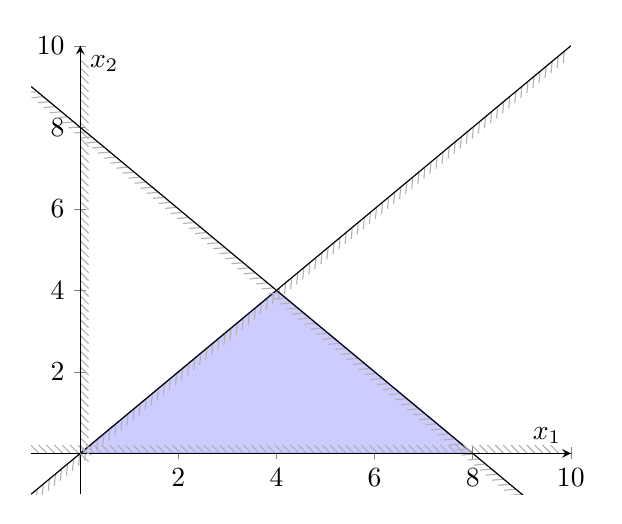
\begin{tikzpicture}
				\begin{axis}[
						axis x line=center,
						axis y line=center,
						xlabel=$x_1$,
						ylabel=$x_2$,
						xmin=-1,
						ymin=-1,
						xmax=10,
						ymax=10,
						xtick={0,2,...,10},
						ytick={0,2,...,10}
					]
					\addplot[fill=blue!20,draw=blue]coordinates{(0,0)(4,4)(8,0)(0,0)};			
					\addPlotLDown{x};
					\addPlotLDown{-x+8}
					\addPlotRUp{0}
		 			\addPlotLDownCoords{(0,0)(0,10)}
				\end{axis}
			\end{tikzpicture}
		\caption{Sample polytope}
	\end{minipage}
\end{figure}

The lp to solve for the chebychev center is

\begin{maxi!}
	{}{r}{}{} 	
	\addConstraint{-1(y_1 + \frac{-1}{\sqrt{2}}r) + (y_2 + \frac{1}{\sqrt{2}}r)}{\leq 0}
	\addConstraint{(y_1 + \frac{-1}{\sqrt{2}}r) + (y_2 + \frac{1}{\sqrt{2}}r)}{\leq 8}
	\addConstraint{y_i}{\geq r}{\quad\forall i \in \{1,2\}}
	\addConstraint{r}{\geq 0}
\end{maxi!}

The optimal objective value is $1.6585$ with $y = \begin{pmatrix}4\\1.65685\end{pmatrix}$


\begin{figure}[h]
	\centering
	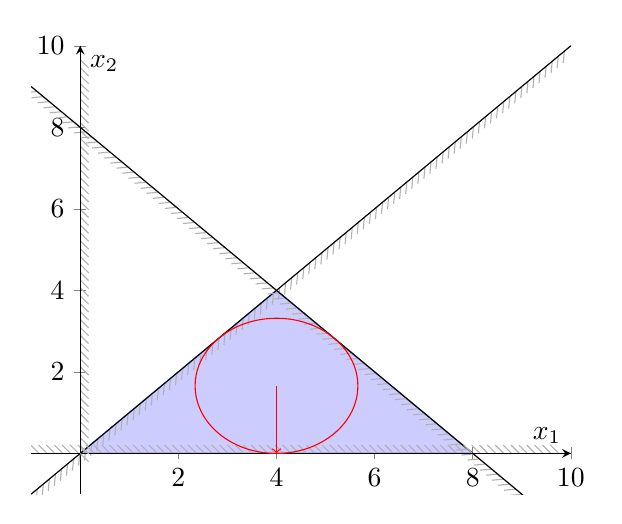
\begin{tikzpicture}
		\begin{axis}[
			axis x line=center,
			axis y line=center,
			xlabel=$x_1$,
			ylabel=$x_2$,
			xmin=-1,
			ymin=-1,
			xmax=10,
			ymax=10,
			xtick={0,2,...,10},
			ytick={0,2,4,6,8,10}
			]
			\addplot[fill=blue!20,draw=blue]coordinates{(0,0)(4,4)(8,0)(0,0)};			
			\addPlotLDown{x};
			\addPlotLDown{-x+8}
			\addPlotRUp{0}
			\addPlotLDownCoords{(0,0)(0,10)}
			\draw [red] (axis cs:4,1.65685) circle [radius=1.6585];
			\draw [->, red] (axis cs:4,1.65685) -- (4,0);
		\end{axis}
	\end{tikzpicture}
	\caption{Sample polytope with chebychev center}
\end{figure}

\subsection{Assume that P has a Chebychev center. Write a linear program for the problem of finding such
a Chebyshev center and the radius of the corresponding ball, and prove that your formulation is
correct. \label{sect:1a}}
See Equation \ref{eq:1}

\subsection{Can the linear program that you found in \(\ref{sect:1a}\) help deciding whether a Chebychev center exists
at all?}
Yes, if there is no Chebychev center at all, the lp becomes unbounded.

\section{Existence of vertices in full-rank polyhedra}
Let $A \in \mathbb{R}^{m \times n}$ have full column rank, let $b \in R^m$ , and consider the polyhedron ${P = \{x \in \mathbb{R}^n : Ax \leq b\}}$
\subsection{For $v, w \in \mathbb{R}^n$ with $w \neq 0$, the set $L(v, w) := \{v + \lambda w : \lambda \in \mathbb{R}\}$ is called a line. Prove that $P$ does
not contain a line, i.e., there are no $v, w \in \mathbb{R}^n$ with $w \neq 0$ such that $L(v, w) \subseteq P$.}

Informal: The Polyhedron is constrained in all variables (because it is a full column rank constrained polyhedron). So there is no possible line since $\lambda$ can be chosen to violate a constraint.

\subsection{Prove that precisely one of the following two statements is true.}
\textit{
		\begin{enumerate}[label=(\roman*)]
		\item $P$ is empty
		\item $P$ has a vertex
	\end{enumerate}
}

Informal: If the polyhedron is not empty, it is at least $2$-dimensional. Therefore the two constraints have to intersect somewhere and form a vertex at the intersection. The same is true for the higher dimensional ones, at least two constraints intersect with each other and form a vertex. 
\end{document}
